%!TEX root = pixelrnn.tex


\section{Experiments}
\label{sect:experiments}

In this section we describe our experiments and results.  We begin by describing the way we evaluate and compare our results. In Section \ref{sect:training_details} we give details about the training. Then we give results on the relative effectiveness of architectural components and our best results on the MNIST, CIFAR-10 and ImageNet datasets.

\subsection{Evaluation}

All our models are trained and evaluated on the log-likelihood loss function coming from a discrete distribution.
Although natural image data is usually modeled with \emph{continuous} distributions using density functions, we can compare our results with previous art in the following way. In the literature it is currently best practice to add real-valued noise to the pixel values to dequantize the data when using density functions \cite{uria2013rnade}. When uniform noise is added (with values in the interval [0, 1]), then the log-likelihoods of continuous and discrete models are directly comparable \cite{theis2015note}. In our case, we can use the values from the discrete distribution as a piecewise-uniform continuous function that has a constant value for every interval $[i, i+1], i = 1, 2, \dots 256$. This corresponding distribution will have the same log-likelihood (on data with added noise) as the original discrete distribution (on discrete data). 

For MNIST we report the negative log-likelihood in \emph{nats} as it is common practice in literature. For CIFAR-10 and ImageNet we report negative log-likelihoods in \emph{bits} per dimension. The total discrete log-likelihood is normalized by the dimensionality of the images (e.g., $32\times 32\times 3=3072$ for CIFAR-10). These numbers are interpretable as the number of bits that a compression scheme based on this model would need to compress every RGB color value \mbox{\citep{van2014student, theis2015note}}; in practice there is also a small overhead due to arithmetic coding.


\subsection{Training Details}
\label{sect:training_details}

Our models are trained on GPUs using the Torch toolbox. From the different parameter update rules tried, RMSProp gives best convergence performance and is used for all experiments. The learning rate schedules were manually set for every dataset to the highest values that allowed fast convergence. The batch sizes also vary for different datasets. For smaller datasets such as MNIST and CIFAR-10 we use smaller batch sizes of 16 images as this seems to regularize the models. For ImageNet we use as large a batch size as allowed by the GPU memory; this corresponds to 64 images/batch for $32\times32$ ImageNet, and 32 images/batch for $64\times64$ ImageNet. Apart from scaling and centering the images at the input of the network, we don't use any other preprocessing or augmentation. For the multinomial loss function we use the raw pixel color values as categories. For all the PixelRNN models, we learn the initial recurrent state of the network.

\subsection{Discrete Softmax Distribution}
Apart from being intuitive and easy to implement, we find that using a softmax on discrete pixel values instead of a mixture density approach on continuous pixel values gives better results. For the Row LSTM model with a softmax output distribution we obtain 3.06 bits/dim on the CIFAR-10 validation set. For the same model with a Mixture of Conditional Gaussian Scale Mixtures (MCGSM) \cite{theis2015generative} we obtain 3.22 bits/dim. % 8052

In Figure \ref{fig:softmax_activations} we show a few softmax activations from the model. Although we don't embed prior information about the meaning or relations of the 256 color categories, e.g. that pixel values 51 and 52 are neighbors, the distributions predicted by the model are meaningful and can be multimodal, skewed, peaked or long tailed. Also note that values 0 and 255 often get a much higher probability as they are more frequent. Another advantage of the discrete distribution is that we do not worry about parts of the distribution mass lying outside the interval [0, 255], which is something that typically happens with continuous distributions.

% \begin{figure}[h]
%   \centering
%   \includegraphics[width=0.48\textwidth]{softmax_new.pdf}
%   \vspace{-0.5cm}
%   \caption{Example softmax activations from the model. The leftmost shows the distribution of the first pixel red value (first value to sample).}
%   \label{fig:softmax_activations}
% \end{figure}
\begin{figure}[h]
  \centering
  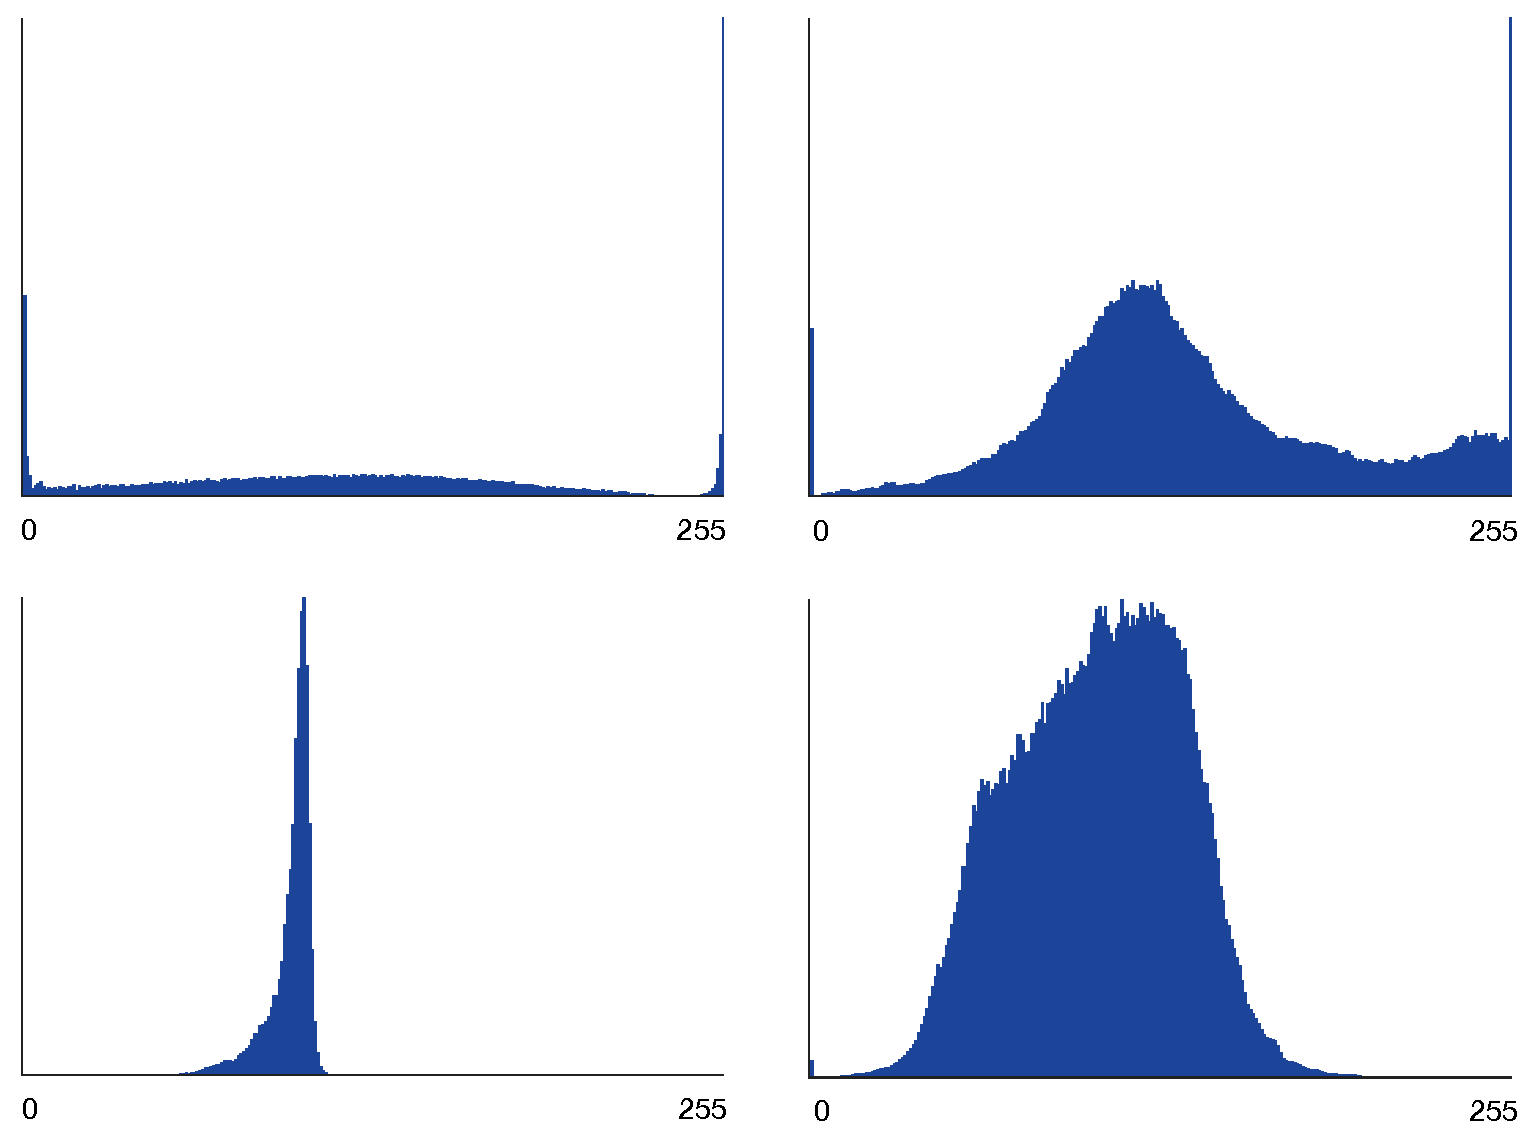
\includegraphics[width=0.48\textwidth]{softmax.pdf}
  \vspace{-0.5cm}
  \caption{Example softmax activations from the model. The top left shows the distribution of the first pixel red value (first value to sample).}
  \label{fig:softmax_activations}
\end{figure}

\begin{figure*}[ht]
\begin{subfigure}{.5\textwidth}
  \centering
  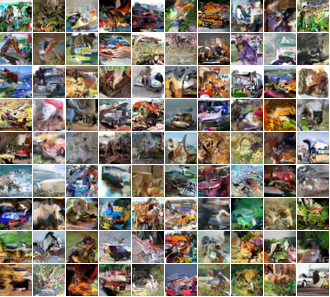
\includegraphics[trim={0 0 0 0},clip, width=0.95\linewidth]{cifar_samples_bilstm_nl5_nh256_cropped.png}
\end{subfigure}%
\hfill
\begin{subfigure}{.5\textwidth}
  \centering
  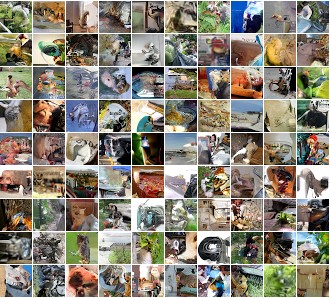
\includegraphics[trim={0 0 0 0},clip, width=0.95\linewidth]{imnet32_samples_residual_nh384_cropped.png}
\end{subfigure}%
\hfill
\caption{Samples from models trained on CIFAR-10 (left) and ImageNet 32x32 (right) images. In general we can see that the models capture local spatial dependencies relatively well. The ImageNet model seems to be better at capturing more global structures than the CIFAR-10 model. The ImageNet model was larger and trained on much more data, which explains the qualitative difference in samples.}
\label{fig:samples_32}
\end{figure*}

\subsection{Residual Connections}
Another core component of the networks is residual connections. In Table \ref{table:effect_skipconnections} we show the results of having residual connections, having standard skip connections or having both, in the 12-layer CIFAR-10 Row LSTM model. We see that using residual connections is as effective as using skip connections; using both is also effective and preserves the advantage. 

\begin{table}[h]
	\begin{center}
	\begin{tabular}{ccc}
		\toprule
		 & \textbf{No skip} & \textbf{Skip} \\ 
		\midrule
		\textbf{No residual}: & 3.22 & 3.09 \\ 
	    \textbf{Residual}: & 3.07 & 3.06 \\ 
	    \bottomrule
	\end{tabular}
	\end{center}
\vspace{-0.3cm}
\caption{Effect of residual and skip connections in the Row LSTM network evaluated on the Cifar-10 validation set in bits/dim.}
\label{table:effect_skipconnections}
\end{table}

When using both the residual and skip connections, we see in Table \ref{table:effect_of_layers} that performance of the Row LSTM improves with increased depth. This holds for up to the 12 LSTM layers that we tried.

\begin{table}[h]
\centering
	\begin{tabular}{ccccccc}
		\toprule
		\textbf{\# layers}: & 1 & 2 & 3 & 6 & 9 & 12 \\ 
	    \midrule
	    \textbf{NLL}: & 3.30 & 3.20 & 3.17 & 3.09 & 3.08 & 3.06 \\
	    \bottomrule
	\end{tabular}
\caption{Effect of the number of layers on the negative log likelihood evaluated on the CIFAR-10 validation set (bits/dim).}
\label{table:effect_of_layers}
\end{table}

\subsection{MNIST}

Although the goal of our work was to model natural images on a large scale, we also tried our model on the binary version \cite{salakhutdinov2008quantitative} of MNIST \cite{lecun1998gradient} as it is a good sanity check and there is a lot of previous art on this dataset to compare with. In Table \ref{table:mnist} we report the performance of the Diagonal BiLSTM model and that of previous published results. To our knowledge this is the best reported result on MNIST so far. 

\begin{table}[!h]
	\begin{center}
	\begin{tabular}{lcc}
		\toprule
		\textbf{Model} & \textbf{NLL Test}  \\ 
		\midrule
		DBM 2hl [1]: & $\approx$ 84.62 \\ 
		DBN 2hl [2]: & $\approx$ 84.55 \\ 
		NADE [3]: & 88.33 \\ 
		EoNADE 2hl (128 orderings) [3]: & 85.10 \\ 
		EoNADE-5 2hl (128 orderings) [4]: \quad \quad \quad & 84.68 \\ 
		DLGM [5]: & $\approx$ 86.60 \\ 
		DLGM 8 leapfrog steps [6]: & $\approx$ 85.51 \\ 
		DARN 1hl [7]: & $\approx$ 84.13 \\ 
		MADE 2hl (32 masks) [8]: & 86.64 \\
		DRAW [9]: & $\leq$ 80.97 \\ 
		\midrule
		PixelCNN: & 81.30 \\ 
		Row LSTM: & 80.54 \\ 
		Diagonal BiLSTM (1 layer, $h=32$): & \textbf{80.75} \\
		Diagonal BiLSTM (7 layers, $h=16$): & \textbf{79.20} \\ 
	    \bottomrule
	\end{tabular}
	\end{center}
\vspace{-0.2cm}
\caption{Test set performance of different models on MNIST in \emph{nats} (negative log-likelihood). Prior results taken from [1] \cite{salakhutdinov2009deep}, [2] \cite{murray2009evaluating}, [3] \cite{uria2013deep}, [4] \cite{raiko2014iterative}, [5] \cite{rezende2014stochastic}, [6] \cite{salimans2014markov}, [7] \cite{gregor2013deep}, [8] \cite{germain2015made}, [9] \cite{gregor2015draw}.}
\label{table:mnist}
\end{table}

\begin{table}[!h]
\centering
	\begin{tabular}{lcc}
		\toprule
		\textbf{Model} & \textbf{NLL Test (Train)}  \\ 
		\midrule
		Uniform Distribution: & 8.00 \\ 
		Multivariate Gaussian: & 4.70 \\ 
		NICE [1]: & 4.48 \\ 
		Deep Diffusion [2]: & 4.20 \\ 
		Deep GMMs [3]: & 4.00 \\
		RIDE [4]: & 3.47 \\ 
		\midrule
		PixelCNN: & 3.14 (3.08) \\ 
		Row LSTM: & 3.07 (3.00) \\ 
		Diagonal BiLSTM: \quad\quad\quad\quad\quad\quad\quad & \textbf{3.00} (2.93) \\ 
	    \bottomrule
	\end{tabular}
\caption{Test set performance of different models on CIFAR-10 in \emph{bits/dim}. For our models we give training performance in brackets. [1] \cite{dinh2014nice}, [2] \cite{deepdiffusion}, [3] \cite{van2014factoring}, [4] personal communication \cite{theis2015generative}.}
\label{table:cifar10}
\end{table}

\begin{table}[!h]
	\begin{center}
	\begin{tabular}{lcc}
		\toprule
		\textbf{Image size} & \textbf{NLL Validation (Train)}  \\ 
		\midrule
		32x32: & 3.86 (3.83) \\ 
		64x64: & 3.63 (3.57) \\ 
	    \bottomrule
	\end{tabular}
	\end{center}
\vspace{-0.2cm}
\caption{Negative log-likelihood performance on $32\times32$ and $64\times64$ ImageNet in \emph{bits/dim}.}
\label{table:imagenet}
\vspace{-0.4cm}
\end{table}


\begin{figure*}[ht]

\begin{subfigure}{.5\textwidth}
  \centering
  % \includegraphics[trim={0 196 521 0},clip, width=0.95\textwidth]{samples_ims64_nl3_nh500.png}
  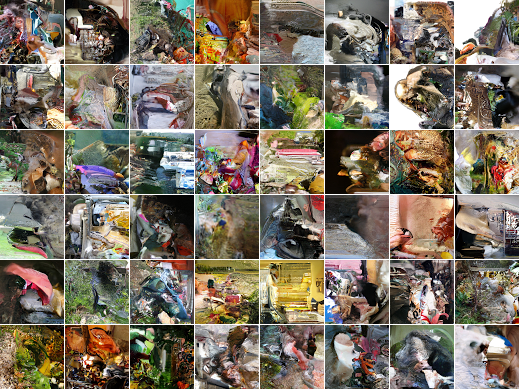
\includegraphics[trim={0 0 0 0},clip, width=0.95\textwidth]{samples_ims64_nl3_nh500_cropped.png}
\end{subfigure}%
\hfill
\begin{subfigure}{.5\textwidth}
  \centering
  % \includegraphics[trim={0 261 1 0},clip, width=0.95\linewidth]{ims64_multiscale.png}
  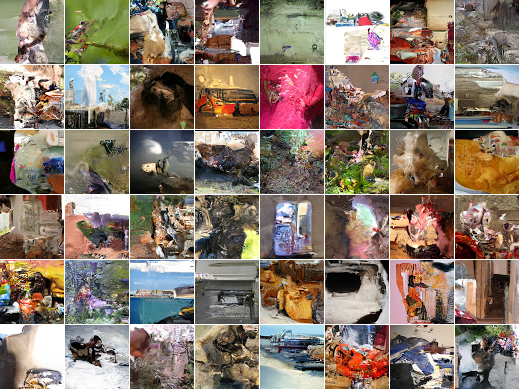
\includegraphics[trim={0 0 0 0},clip, width=0.95\linewidth]{ims64_multiscale_cropped.png}
\end{subfigure}%
\hfill
\caption{Samples from models trained on ImageNet 64x64 images. Left: normal model, right: multi-scale model. The single-scale model trained on 64x64 images is less able to capture global structure than the 32x32 model. The multi-scale model seems to resolve this problem. Although these models get similar performance in log-likelihood, the samples on the right do seem globally more coherent.}
\label{fig:samples_64}
\end{figure*}

\subsection{CIFAR-10}

Next we test our models on the CIFAR-10 dataset \cite{krizhevsky2009learning}. Table \ref{table:cifar10} lists the results of our models and that of previously published approaches. All our results were obtained without data augmentation. For the proposed networks, the Diagonal BiLSTM has the best performance, followed by the Row LSTM and the PixelCNN. This coincides with the size of the respective receptive fields: the Diagonal BiLSTM has a global view, the Row LSTM has a partially occluded view and the PixelCNN sees the fewest pixels in the context. This suggests that effectively capturing a large receptive field is important. 
Figure \ref{fig:samples_32} (left) shows CIFAR-10 samples generated from the Diagonal BiLSTM.

\begin{figure}[!ht]
\centering
\hspace{0.02cm} {occluded} \hfill completions \hfill{original} \,
\vspace{0.1cm}
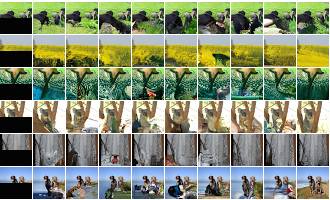
\includegraphics[width=\linewidth]{compl1_2.png}
\vspace{-0.5cm}
\caption{Image completions sampled from a model that was trained on 32x32 ImageNet images. Note that diversity of the completions is high, which can be attributed to the log-likelihood loss function used in this generative model, as it encourages models with high entropy. As these are sampled from the model, we can easily generate millions of different completions. It is also interesting to see that textures such as water, wood and shrubbery are also inputed relative well (see Figure \ref{fig:intro_completions}).}
\label{fig:completions}
\vspace{-0.2cm}
\end{figure}
% \begin{figure*}[!ht]
% \begin{subfigure}{.5\textwidth}
%   \centering
% \hspace{0.02cm} {occluded} \hfill completions \hfill{original} \,

% \vspace{0.1cm}
%   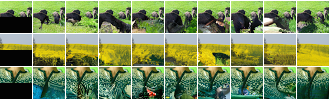
\includegraphics[width=0.96\textwidth]{compl2.png}
% \end{subfigure}%
% \hfill
% \begin{subfigure}{.5\textwidth}
%   \centering
% \hspace{0.02cm} {occluded} \hfill completions \hfill{original} \,

% \vspace{0.1cm}
%   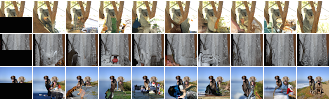
\includegraphics[ width=0.96\linewidth]{compl1.png}
% \end{subfigure}%
% \hfill
% \caption{Image completions sampled from a model that was trained on 32x32 ImageNet images. Note that diversity of the completions is high, which can be attributed to the log-likelihood loss function used in this generative model, as it encourages models with high entropy. As these are sampled from the model, we can easily generate millions of different completions. It is also interesting to see that textures such as water, wood and shrubbery are also inputed relative well (see Figure \ref{fig:intro_completions}).}
% \label{fig:completions}
% \vspace{-0.2cm}
% \end{figure*}

\vspace{0.4cm}
\subsection{ImageNet}

Although to our knowledge the are no published results on the ILSVRC ImageNet dataset \cite{ILSVRC15} that we can compare our models with, we give our ImageNet log-likelihood performance in Table \ref{table:imagenet} (without data augmentation). On ImageNet the current PixelRNNs do not appear to overfit, as we saw that their validation performance improved with size and depth. The main constraint on model size are currently computation time and GPU memory.

Note that the ImageNet models are in general less compressible than the CIFAR-10 images. ImageNet has greater variety of images, and the CIFAR-10 images were most likely resized with a different algorithm than the one we used for ImageNet images. The ImageNet images are less blurry, which means neighboring pixels are less correlated to each other and thus less predictable. Because the downsampling method can influence the compression performance, we have made the used downsampled images available\footnote{http://image-net.org/small/download.php}.

Figure \ref{fig:samples_32} (right) shows $32\times32$ samples drawn from our model trained on ImageNet. Figure \ref{fig:samples_64} shows $64\times64$ samples from the same model with and without multi-scale conditioning. Finally, we also show image completions sampled from the model in Figure \ref{fig:completions}.






